\documentclass{book}
\usepackage[a4paper,top=2.5cm,bottom=2.5cm,left=2.5cm,right=2.5cm]{geometry}
\usepackage{makeidx}
\usepackage{natbib}
\usepackage{graphicx}
\usepackage{multicol}
\usepackage{float}
\usepackage{listings}
\usepackage{color}
\usepackage{ifthen}
\usepackage[table]{xcolor}
\usepackage{textcomp}
\usepackage{alltt}
\usepackage{ifpdf}
\ifpdf
\usepackage[pdftex,
            pagebackref=true,
            colorlinks=true,
            linkcolor=blue,
            unicode
           ]{hyperref}
\else
\usepackage[ps2pdf,
            pagebackref=true,
            colorlinks=true,
            linkcolor=blue,
            unicode
           ]{hyperref}
\usepackage{pspicture}
\fi
\usepackage[utf8]{inputenc}
\usepackage{mathptmx}
\usepackage[scaled=.90]{helvet}
\usepackage{courier}
\usepackage{sectsty}
\usepackage{amssymb}
\usepackage[titles]{tocloft}
\usepackage{doxygen}
\lstset{language=C++,inputencoding=utf8,basicstyle=\footnotesize,breaklines=true,breakatwhitespace=true,tabsize=2,numbers=left }
\makeindex
\setcounter{tocdepth}{3}
\renewcommand{\footrulewidth}{0.4pt}
\renewcommand{\familydefault}{\sfdefault}
\hfuzz=15pt
\setlength{\emergencystretch}{15pt}
\hbadness=750
\tolerance=750
\begin{document}
\hypersetup{pageanchor=false,citecolor=blue}
\begin{titlepage}
\vspace*{7cm}
\begin{center}
{\Large Boost\-D\-S\-P }\\
\vspace*{1cm}
{\large Generated by Doxygen 1.8.3.1}\\
\vspace*{0.5cm}
{\small Fri Sep 20 2013 18:40:52}\\
\end{center}
\end{titlepage}
\clearemptydoublepage
\pagenumbering{roman}
\tableofcontents
\clearemptydoublepage
\pagenumbering{arabic}
\hypersetup{pageanchor=true,citecolor=blue}
\chapter{Design Unit Index}
\section{Design Unit Hierarchy}
This inheritance list is sorted roughly, but not completely, alphabetically\-:\begin{DoxyCompactList}
\item \contentsline{section}{lfsr\-\_\-internal}{\pageref{classlfsr__internal}}{}
\item \contentsline{section}{lfsr\-\_\-tb}{\pageref{classlfsr__tb}}{}
\begin{DoxyCompactList}
\item \contentsline{section}{lfsr}{\pageref{classlfsr}}{}
\end{DoxyCompactList}
\end{DoxyCompactList}

\chapter{Design Unit Index}
\section{Design Unit List}
Here is a list of all design unit members with links to the Entities they belong to\-:\begin{DoxyCompactList}
\item\contentsline{section}{architecture \hyperlink{classlfsr_1_1beh}{beh} }{\pageref{classlfsr_1_1beh}}{}
\item\contentsline{section}{architecture \hyperlink{classlfsr__internal_1_1direct}{direct} }{\pageref{classlfsr__internal_1_1direct}}{}
\item\contentsline{section}{architecture \hyperlink{classlfsr__internal_1_1galois}{galois} }{\pageref{classlfsr__internal_1_1galois}}{}
\item\contentsline{section}{entity \hyperlink{classlfsr}{lfsr} }{\pageref{classlfsr}}{}
\item\contentsline{section}{entity \hyperlink{classlfsr__internal}{lfsr\-\_\-internal} }{\pageref{classlfsr__internal}}{}
\item\contentsline{section}{entity \hyperlink{classlfsr__tb}{lfsr\-\_\-tb} }{\pageref{classlfsr__tb}}{}
\item\contentsline{section}{architecture \hyperlink{classlfsr__tb_1_1sim}{sim} }{\pageref{classlfsr__tb_1_1sim}}{}
\end{DoxyCompactList}

\chapter{Class Documentation}
\hypertarget{class__lfsr__pkg}{\section{lfsr\-\_\-pkg Package Body Reference}
\label{class__lfsr__pkg}\index{lfsr\-\_\-pkg@{lfsr\-\_\-pkg}}
}
{\bfseries Package $>$$>$ }\hyperlink{classlfsr__pkg}{lfsr\-\_\-pkg}\\*
\subsection*{Functions}
 \begin{DoxyCompactItemize}
\item 
\hypertarget{class__lfsr__pkg_aa892d93dafd63bb0a40765dec3e73940}{{\bfseries {\bfseries \textcolor{comment}{std\-\_\-logic\-\_\-vector}\textcolor{vhdlchar}{ }}} \hyperlink{class__lfsr__pkg_aa892d93dafd63bb0a40765dec3e73940}{Maximal\-\_\-\-Polynomial}{\bfseries  ( }{\bfseries \textcolor{vhdlchar}{size\-: }\textcolor{stringliteral}{in }\textcolor{vhdlchar}{positive}}{\bfseries  )} }\label{class__lfsr__pkg_aa892d93dafd63bb0a40765dec3e73940}

\end{DoxyCompactItemize}


The documentation for this class was generated from the following file\-:\begin{DoxyCompactItemize}
\item 
src/lfsr/lfsr\-\_\-pkg.\-vhd\end{DoxyCompactItemize}

\hypertarget{class__util__pkg}{\section{util\-\_\-pkg Package Body Reference}
\label{class__util__pkg}\index{util\-\_\-pkg@{util\-\_\-pkg}}
}
{\bfseries Package $>$$>$ }\hyperlink{classutil__pkg}{util\-\_\-pkg}\\*
\subsection*{Functions}
 \begin{DoxyCompactItemize}
\item 
\hypertarget{class__util__pkg_a75d57d42f413f4f44fe472e114c76b50}{{\bfseries {\bfseries \textcolor{comment}{integer}\textcolor{vhdlchar}{ }}} \hyperlink{class__util__pkg_a75d57d42f413f4f44fe472e114c76b50}{max}{\bfseries  ( }{\bfseries \textcolor{vhdlchar}{i\-: }\textcolor{stringliteral}{in }{\bfseries \textcolor{comment}{integer}\textcolor{vhdlchar}{ }}}{\bfseries  , \textcolor{vhdlchar}{j\-: }\textcolor{stringliteral}{in }{\bfseries \textcolor{comment}{integer}\textcolor{vhdlchar}{ }}}{\bfseries  )} }\label{class__util__pkg_a75d57d42f413f4f44fe472e114c76b50}

\item 
\hypertarget{class__util__pkg_a9abf89c3351a7e2c76ffa1943ab815e0}{{\bfseries {\bfseries \textcolor{comment}{std\-\_\-logic\-\_\-vector}\textcolor{vhdlchar}{ }}} \hyperlink{class__util__pkg_a9abf89c3351a7e2c76ffa1943ab815e0}{reverse}{\bfseries  ( }{\bfseries \textcolor{vhdlchar}{x\-: }\textcolor{stringliteral}{in }{\bfseries \textcolor{comment}{std\-\_\-logic\-\_\-vector}\textcolor{vhdlchar}{ }}}{\bfseries  )} }\label{class__util__pkg_a9abf89c3351a7e2c76ffa1943ab815e0}

\end{DoxyCompactItemize}


The documentation for this class was generated from the following file\-:\begin{DoxyCompactItemize}
\item 
src/util\-\_\-pkg.\-vhd\end{DoxyCompactItemize}

\hypertarget{classlfsr_1_1beh}{\section{beh Architecture Reference}
\label{classlfsr_1_1beh}\index{beh@{beh}}
}
\subsection*{Components}
 \begin{DoxyCompactItemize}
\item 
\hypertarget{classlfsr_1_1beh_a6372737c0851c0a5e0070813196d076b}{\hyperlink{classlfsr_1_1beh_a6372737c0851c0a5e0070813196d076b}{lfsr\-\_\-internal}  {\bfseries }  }\label{classlfsr_1_1beh_a6372737c0851c0a5e0070813196d076b}

\end{DoxyCompactItemize}


The documentation for this class was generated from the following file\-:\begin{DoxyCompactItemize}
\item 
src/lfsr/lfsr.\-vhd\end{DoxyCompactItemize}

\hypertarget{classlfsr__internal_1_1direct}{\section{direct Architecture Reference}
\label{classlfsr__internal_1_1direct}\index{direct@{direct}}
}
\subsection*{Processes}
 \begin{DoxyCompactItemize}
\item 
\hypertarget{classlfsr__internal_1_1direct_ab0a54e92d710dc996e125e7c3c005889}{\hyperlink{classlfsr__internal_1_1direct_ab0a54e92d710dc996e125e7c3c005889}{data\-\_\-pipeline}{\bfseries  ( {\bfseries \textcolor{vhdlchar}{clk}\textcolor{vhdlchar}{ }\textcolor{vhdlchar}{ }\textcolor{vhdlchar}{ }} , {\bfseries \textcolor{vhdlchar}{rst}\textcolor{vhdlchar}{ }} )}}\label{classlfsr__internal_1_1direct_ab0a54e92d710dc996e125e7c3c005889}

\end{DoxyCompactItemize}
\subsection*{Constants}
 \begin{DoxyCompactItemize}
\item 
\hypertarget{classlfsr__internal_1_1direct_a2da9a4fd5d161e082e10adfe2b4045b0}{\hyperlink{classlfsr__internal_1_1direct_a2da9a4fd5d161e082e10adfe2b4045b0}{W\-I\-D\-T\-H} {\bfseries \textcolor{vhdlchar}{positive}\textcolor{vhdlchar}{ }\textcolor{vhdlchar}{ }\textcolor{vhdlchar}{\-:}\textcolor{vhdlchar}{=}\textcolor{vhdlchar}{ }\textcolor{vhdlchar}{max}\textcolor{vhdlchar}{ }\textcolor{vhdlchar}{(}\textcolor{vhdlchar}{ }\textcolor{vhdlchar}{ }\textcolor{vhdlchar}{max}\textcolor{vhdlchar}{ }\textcolor{vhdlchar}{(}\textcolor{vhdlchar}{ }\textcolor{vhdlchar}{ } \textcolor{vhdldigit}{2} \textcolor{vhdlchar}{ }\textcolor{vhdlchar}{,}\textcolor{vhdlchar}{ }\textcolor{vhdlchar}{ }\textcolor{vhdlchar}{I\-N\-T\-E\-R\-N\-A\-L\-\_\-\-S\-I\-Z\-E}\textcolor{vhdlchar}{ }\textcolor{vhdlchar}{)}\textcolor{vhdlchar}{ }\textcolor{vhdlchar}{ }\textcolor{vhdlchar}{,}\textcolor{vhdlchar}{ }\textcolor{vhdlchar}{ }\textcolor{vhdlchar}{q}\textcolor{vhdlchar}{ }\textcolor{vhdlchar}{'}\textcolor{vhdlchar}{ }\textcolor{vhdlchar}{ }\textcolor{vhdlchar}{length}\textcolor{vhdlchar}{ }\textcolor{vhdlchar}{)}\textcolor{vhdlchar}{ }} }\label{classlfsr__internal_1_1direct_a2da9a4fd5d161e082e10adfe2b4045b0}

\item 
\hypertarget{classlfsr__internal_1_1direct_a3d02278b409147fbd08ccc73659770dc}{\hyperlink{classlfsr__internal_1_1direct_a3d02278b409147fbd08ccc73659770dc}{poly} {\bfseries \textcolor{vhdlchar}{int\-\_\-reg\-\_\-type}\textcolor{vhdlchar}{ }\textcolor{vhdlchar}{ }\textcolor{vhdlchar}{\-:}\textcolor{vhdlchar}{=}\textcolor{vhdlchar}{ }\textcolor{vhdlchar}{Maximal\-\_\-\-Polynomial}\textcolor{vhdlchar}{ }\textcolor{vhdlchar}{(}\textcolor{vhdlchar}{ }\textcolor{vhdlchar}{ }\textcolor{vhdlchar}{W\-I\-D\-T\-H}\textcolor{vhdlchar}{ }\textcolor{vhdlchar}{)}\textcolor{vhdlchar}{ }} }\label{classlfsr__internal_1_1direct_a3d02278b409147fbd08ccc73659770dc}

\item 
\hypertarget{classlfsr__internal_1_1direct_a8977b25492c57870937c271c9ca7f817}{\hyperlink{classlfsr__internal_1_1direct_a8977b25492c57870937c271c9ca7f817}{reverse\-\_\-poly} {\bfseries \textcolor{vhdlchar}{int\-\_\-reg\-\_\-type}\textcolor{vhdlchar}{ }\textcolor{vhdlchar}{ }\textcolor{vhdlchar}{\-:}\textcolor{vhdlchar}{=}\textcolor{vhdlchar}{ }\textcolor{vhdlchar}{reverse}\textcolor{vhdlchar}{ }\textcolor{vhdlchar}{(}\textcolor{vhdlchar}{ }\textcolor{vhdlchar}{ }\textcolor{vhdlchar}{poly}\textcolor{vhdlchar}{ }\textcolor{vhdlchar}{)}\textcolor{vhdlchar}{ }} }\label{classlfsr__internal_1_1direct_a8977b25492c57870937c271c9ca7f817}

\item 
\hypertarget{classlfsr__internal_1_1direct_ab70454a2af1f27e2eabaaacd9288b1a1}{\hyperlink{classlfsr__internal_1_1direct_ab70454a2af1f27e2eabaaacd9288b1a1}{B\-A\-D\-\_\-\-S\-E\-E\-D} {\bfseries \textcolor{vhdlchar}{int\-\_\-reg\-\_\-type}\textcolor{vhdlchar}{ }\textcolor{vhdlchar}{ }\textcolor{vhdlchar}{\-:}\textcolor{vhdlchar}{=}\textcolor{vhdlchar}{ }\textcolor{vhdlchar}{(}\textcolor{vhdlchar}{ }\textcolor{vhdlchar}{ }\textcolor{vhdlkeyword}{others}\textcolor{vhdlchar}{ }\textcolor{vhdlchar}{ }\textcolor{vhdlchar}{=}\textcolor{vhdlchar}{ }\textcolor{vhdlchar}{$>$}\textcolor{vhdlchar}{ }\textcolor{vhdlchar}{'}\textcolor{vhdlchar}{ } \textcolor{vhdldigit}{1} \textcolor{vhdlchar}{ }\textcolor{vhdlchar}{'}\textcolor{vhdlchar}{ }\textcolor{vhdlchar}{ }\textcolor{vhdlchar}{)}\textcolor{vhdlchar}{ }} }\label{classlfsr__internal_1_1direct_ab70454a2af1f27e2eabaaacd9288b1a1}

\end{DoxyCompactItemize}
\subsection*{Subtypes}
 \begin{DoxyCompactItemize}
\item 
\hypertarget{classlfsr__internal_1_1direct_ac2858aa29a2e169c0b30226c11d09588}{\hyperlink{classlfsr__internal_1_1direct_ac2858aa29a2e169c0b30226c11d09588}{int\-\_\-range} {\bfseries \textcolor{comment}{natural}\textcolor{vhdlchar}{ }\textcolor{vhdlkeyword}{range}\textcolor{vhdlchar}{ }\textcolor{vhdlchar}{(}\textcolor{vhdlchar}{ }\textcolor{vhdlchar}{W\-I\-D\-T\-H}\textcolor{vhdlchar}{ }\textcolor{vhdlchar}{-\/}\textcolor{vhdlchar}{ } \textcolor{vhdldigit}{1} \textcolor{vhdlchar}{ }\textcolor{vhdlchar}{)}\textcolor{vhdlchar}{ }\textcolor{vhdlchar}{ }\textcolor{vhdlchar}{ }\textcolor{vhdlchar}{ }\textcolor{vhdlkeyword}{downto}\textcolor{vhdlchar}{ }\textcolor{vhdlchar}{ }\textcolor{vhdlchar}{ } \textcolor{vhdldigit}{0} \textcolor{vhdlchar}{ }} }\label{classlfsr__internal_1_1direct_ac2858aa29a2e169c0b30226c11d09588}

\item 
\hypertarget{classlfsr__internal_1_1direct_a03558613996994534b7cf3c7aa4ee07e}{\hyperlink{classlfsr__internal_1_1direct_a03558613996994534b7cf3c7aa4ee07e}{int\-\_\-reg\-\_\-type} {\bfseries \textcolor{comment}{std\-\_\-logic\-\_\-vector}\textcolor{vhdlchar}{ }\textcolor{vhdlchar}{(}\textcolor{vhdlchar}{ }\textcolor{vhdlchar}{ }\textcolor{vhdlchar}{int\-\_\-range}\textcolor{vhdlchar}{ }\textcolor{vhdlchar}{)}\textcolor{vhdlchar}{ }} }\label{classlfsr__internal_1_1direct_a03558613996994534b7cf3c7aa4ee07e}

\end{DoxyCompactItemize}
\subsection*{Signals}
 \begin{DoxyCompactItemize}
\item 
\hypertarget{classlfsr__internal_1_1direct_a3ecfc79e7dbfac52489805f58aabae21}{\hyperlink{classlfsr__internal_1_1direct_a3ecfc79e7dbfac52489805f58aabae21}{lfsr\-\_\-reg} {\bfseries \textcolor{vhdlchar}{int\-\_\-reg\-\_\-type}\textcolor{vhdlchar}{ }\textcolor{vhdlchar}{ }\textcolor{vhdlchar}{\-:}\textcolor{vhdlchar}{=}\textcolor{vhdlchar}{ }\textcolor{comment}{std\-\_\-logic\-\_\-vector}\textcolor{vhdlchar}{ }\textcolor{vhdlchar}{(}\textcolor{vhdlchar}{ }\textcolor{vhdlchar}{ }\textcolor{vhdlchar}{to\-\_\-unsigned}\textcolor{vhdlchar}{ }\textcolor{vhdlchar}{(}\textcolor{vhdlchar}{ }\textcolor{vhdlchar}{ }\textcolor{vhdlchar}{S\-E\-E\-D}\textcolor{vhdlchar}{ }\textcolor{vhdlchar}{,}\textcolor{vhdlchar}{ }\textcolor{vhdlchar}{ }\textcolor{vhdlchar}{W\-I\-D\-T\-H}\textcolor{vhdlchar}{ }\textcolor{vhdlchar}{)}\textcolor{vhdlchar}{ }\textcolor{vhdlchar}{ }\textcolor{vhdlchar}{)}\textcolor{vhdlchar}{ }} }\label{classlfsr__internal_1_1direct_a3ecfc79e7dbfac52489805f58aabae21}

\end{DoxyCompactItemize}


The documentation for this class was generated from the following file\-:\begin{DoxyCompactItemize}
\item 
src/lfsr/lfsr\-\_\-internal\-\_\-ea.\-vhd\end{DoxyCompactItemize}

\hypertarget{classlfsr__internal_1_1galois}{\section{galois Architecture Reference}
\label{classlfsr__internal_1_1galois}\index{galois@{galois}}
}
\subsection*{Processes}
 \begin{DoxyCompactItemize}
\item 
\hypertarget{classlfsr__internal_1_1galois_ab0a54e92d710dc996e125e7c3c005889}{\hyperlink{classlfsr__internal_1_1galois_ab0a54e92d710dc996e125e7c3c005889}{data\-\_\-pipeline}{\bfseries  ( {\bfseries \textcolor{vhdlchar}{clk}\textcolor{vhdlchar}{ }\textcolor{vhdlchar}{ }\textcolor{vhdlchar}{ }} , {\bfseries \textcolor{vhdlchar}{rst}\textcolor{vhdlchar}{ }} )}}\label{classlfsr__internal_1_1galois_ab0a54e92d710dc996e125e7c3c005889}

\end{DoxyCompactItemize}
\subsection*{Constants}
 \begin{DoxyCompactItemize}
\item 
\hypertarget{classlfsr__internal_1_1galois_a75f0efa20cdf98228e8ec37f15405484}{\hyperlink{classlfsr__internal_1_1galois_a75f0efa20cdf98228e8ec37f15405484}{width} {\bfseries \textcolor{vhdlchar}{positive}\textcolor{vhdlchar}{ }\textcolor{vhdlchar}{ }\textcolor{vhdlchar}{\-:}\textcolor{vhdlchar}{=}\textcolor{vhdlchar}{ }\textcolor{vhdlchar}{max}\textcolor{vhdlchar}{ }\textcolor{vhdlchar}{(}\textcolor{vhdlchar}{ }\textcolor{vhdlchar}{ }\textcolor{vhdlchar}{max}\textcolor{vhdlchar}{ }\textcolor{vhdlchar}{(}\textcolor{vhdlchar}{ }\textcolor{vhdlchar}{ } \textcolor{vhdldigit}{2} \textcolor{vhdlchar}{ }\textcolor{vhdlchar}{,}\textcolor{vhdlchar}{ }\textcolor{vhdlchar}{ }\textcolor{vhdlchar}{I\-N\-T\-E\-R\-N\-A\-L\-\_\-\-S\-I\-Z\-E}\textcolor{vhdlchar}{ }\textcolor{vhdlchar}{)}\textcolor{vhdlchar}{ }\textcolor{vhdlchar}{ }\textcolor{vhdlchar}{,}\textcolor{vhdlchar}{ }\textcolor{vhdlchar}{ }\textcolor{vhdlchar}{q}\textcolor{vhdlchar}{ }\textcolor{vhdlchar}{'}\textcolor{vhdlchar}{ }\textcolor{vhdlchar}{ }\textcolor{vhdlchar}{length}\textcolor{vhdlchar}{ }\textcolor{vhdlchar}{)}\textcolor{vhdlchar}{ }} }\label{classlfsr__internal_1_1galois_a75f0efa20cdf98228e8ec37f15405484}

\item 
\hypertarget{classlfsr__internal_1_1galois_a3d02278b409147fbd08ccc73659770dc}{\hyperlink{classlfsr__internal_1_1galois_a3d02278b409147fbd08ccc73659770dc}{poly} {\bfseries \textcolor{vhdlchar}{int\-\_\-reg\-\_\-type}\textcolor{vhdlchar}{ }\textcolor{vhdlchar}{ }\textcolor{vhdlchar}{\-:}\textcolor{vhdlchar}{=}\textcolor{vhdlchar}{ }\textcolor{vhdlchar}{Maximal\-\_\-\-Polynomial}\textcolor{vhdlchar}{ }\textcolor{vhdlchar}{(}\textcolor{vhdlchar}{ }\textcolor{vhdlchar}{ }\textcolor{vhdlchar}{W\-I\-D\-T\-H}\textcolor{vhdlchar}{ }\textcolor{vhdlchar}{)}\textcolor{vhdlchar}{ }} }\label{classlfsr__internal_1_1galois_a3d02278b409147fbd08ccc73659770dc}

\item 
\hypertarget{classlfsr__internal_1_1galois_af2ff8ccf0656e6f01c106f9a9a8b066e}{\hyperlink{classlfsr__internal_1_1galois_af2ff8ccf0656e6f01c106f9a9a8b066e}{B\-A\-D\-\_\-\-S\-E\-E\-D} {\bfseries \textcolor{vhdlchar}{int\-\_\-reg}\textcolor{vhdlchar}{ }\textcolor{vhdlchar}{ }\textcolor{vhdlchar}{\-:}\textcolor{vhdlchar}{=}\textcolor{vhdlchar}{ }\textcolor{vhdlchar}{(}\textcolor{vhdlchar}{ }\textcolor{vhdlchar}{ }\textcolor{vhdlkeyword}{others}\textcolor{vhdlchar}{ }\textcolor{vhdlchar}{ }\textcolor{vhdlchar}{=}\textcolor{vhdlchar}{ }\textcolor{vhdlchar}{$>$}\textcolor{vhdlchar}{ }\textcolor{vhdlchar}{'}\textcolor{vhdlchar}{ } \textcolor{vhdldigit}{1} \textcolor{vhdlchar}{ }\textcolor{vhdlchar}{'}\textcolor{vhdlchar}{ }\textcolor{vhdlchar}{ }\textcolor{vhdlchar}{)}\textcolor{vhdlchar}{ }} }\label{classlfsr__internal_1_1galois_af2ff8ccf0656e6f01c106f9a9a8b066e}

\end{DoxyCompactItemize}
\subsection*{Subtypes}
 \begin{DoxyCompactItemize}
\item 
\hypertarget{classlfsr__internal_1_1galois_ab2d0d8d261d904b93bba56b13edd625e}{\hyperlink{classlfsr__internal_1_1galois_ab2d0d8d261d904b93bba56b13edd625e}{int\-\_\-range} {\bfseries \textcolor{comment}{natural}\textcolor{vhdlchar}{ }\textcolor{vhdlkeyword}{range}\textcolor{vhdlchar}{ }\textcolor{vhdlchar}{(}\textcolor{vhdlchar}{ }\textcolor{vhdlchar}{width}\textcolor{vhdlchar}{ }\textcolor{vhdlchar}{-\/}\textcolor{vhdlchar}{ } \textcolor{vhdldigit}{1} \textcolor{vhdlchar}{ }\textcolor{vhdlchar}{)}\textcolor{vhdlchar}{ }\textcolor{vhdlchar}{ }\textcolor{vhdlchar}{ }\textcolor{vhdlchar}{ }\textcolor{vhdlkeyword}{downto}\textcolor{vhdlchar}{ }\textcolor{vhdlchar}{ }\textcolor{vhdlchar}{ } \textcolor{vhdldigit}{0} \textcolor{vhdlchar}{ }} }\label{classlfsr__internal_1_1galois_ab2d0d8d261d904b93bba56b13edd625e}

\item 
\hypertarget{classlfsr__internal_1_1galois_a2d7c50054760503d0dd91b9baaa48217}{\hyperlink{classlfsr__internal_1_1galois_a2d7c50054760503d0dd91b9baaa48217}{int\-\_\-reg} {\bfseries \textcolor{comment}{std\-\_\-logic\-\_\-vector}\textcolor{vhdlchar}{ }\textcolor{vhdlchar}{(}\textcolor{vhdlchar}{ }\textcolor{vhdlchar}{ }\textcolor{vhdlchar}{int\-\_\-range}\textcolor{vhdlchar}{ }\textcolor{vhdlchar}{)}\textcolor{vhdlchar}{ }} }\label{classlfsr__internal_1_1galois_a2d7c50054760503d0dd91b9baaa48217}

\end{DoxyCompactItemize}
\subsection*{Signals}
 \begin{DoxyCompactItemize}
\item 
\hypertarget{classlfsr__internal_1_1galois_a42727b75ccbd70a3d1f5b053dc4f77de}{\hyperlink{classlfsr__internal_1_1galois_a42727b75ccbd70a3d1f5b053dc4f77de}{lfsr\-\_\-reg} {\bfseries \textcolor{vhdlchar}{int\-\_\-reg}\textcolor{vhdlchar}{ }\textcolor{vhdlchar}{ }\textcolor{vhdlchar}{\-:}\textcolor{vhdlchar}{=}\textcolor{vhdlchar}{ }\textcolor{comment}{std\-\_\-logic\-\_\-vector}\textcolor{vhdlchar}{ }\textcolor{vhdlchar}{(}\textcolor{vhdlchar}{ }\textcolor{vhdlchar}{ }\textcolor{vhdlchar}{to\-\_\-unsigned}\textcolor{vhdlchar}{ }\textcolor{vhdlchar}{(}\textcolor{vhdlchar}{ }\textcolor{vhdlchar}{ }\textcolor{vhdlchar}{S\-E\-E\-D}\textcolor{vhdlchar}{ }\textcolor{vhdlchar}{,}\textcolor{vhdlchar}{ }\textcolor{vhdlchar}{ }\textcolor{vhdlchar}{width}\textcolor{vhdlchar}{ }\textcolor{vhdlchar}{)}\textcolor{vhdlchar}{ }\textcolor{vhdlchar}{ }\textcolor{vhdlchar}{)}\textcolor{vhdlchar}{ }} }\label{classlfsr__internal_1_1galois_a42727b75ccbd70a3d1f5b053dc4f77de}

\end{DoxyCompactItemize}


The documentation for this class was generated from the following file\-:\begin{DoxyCompactItemize}
\item 
src/lfsr/lfsr\-\_\-internal\-\_\-ea.\-vhd\end{DoxyCompactItemize}

\hypertarget{classlfsr}{\section{lfsr Entity Reference}
\label{classlfsr}\index{lfsr@{lfsr}}
}
Inheritance diagram for lfsr\-:\begin{figure}[H]
\begin{center}
\leavevmode
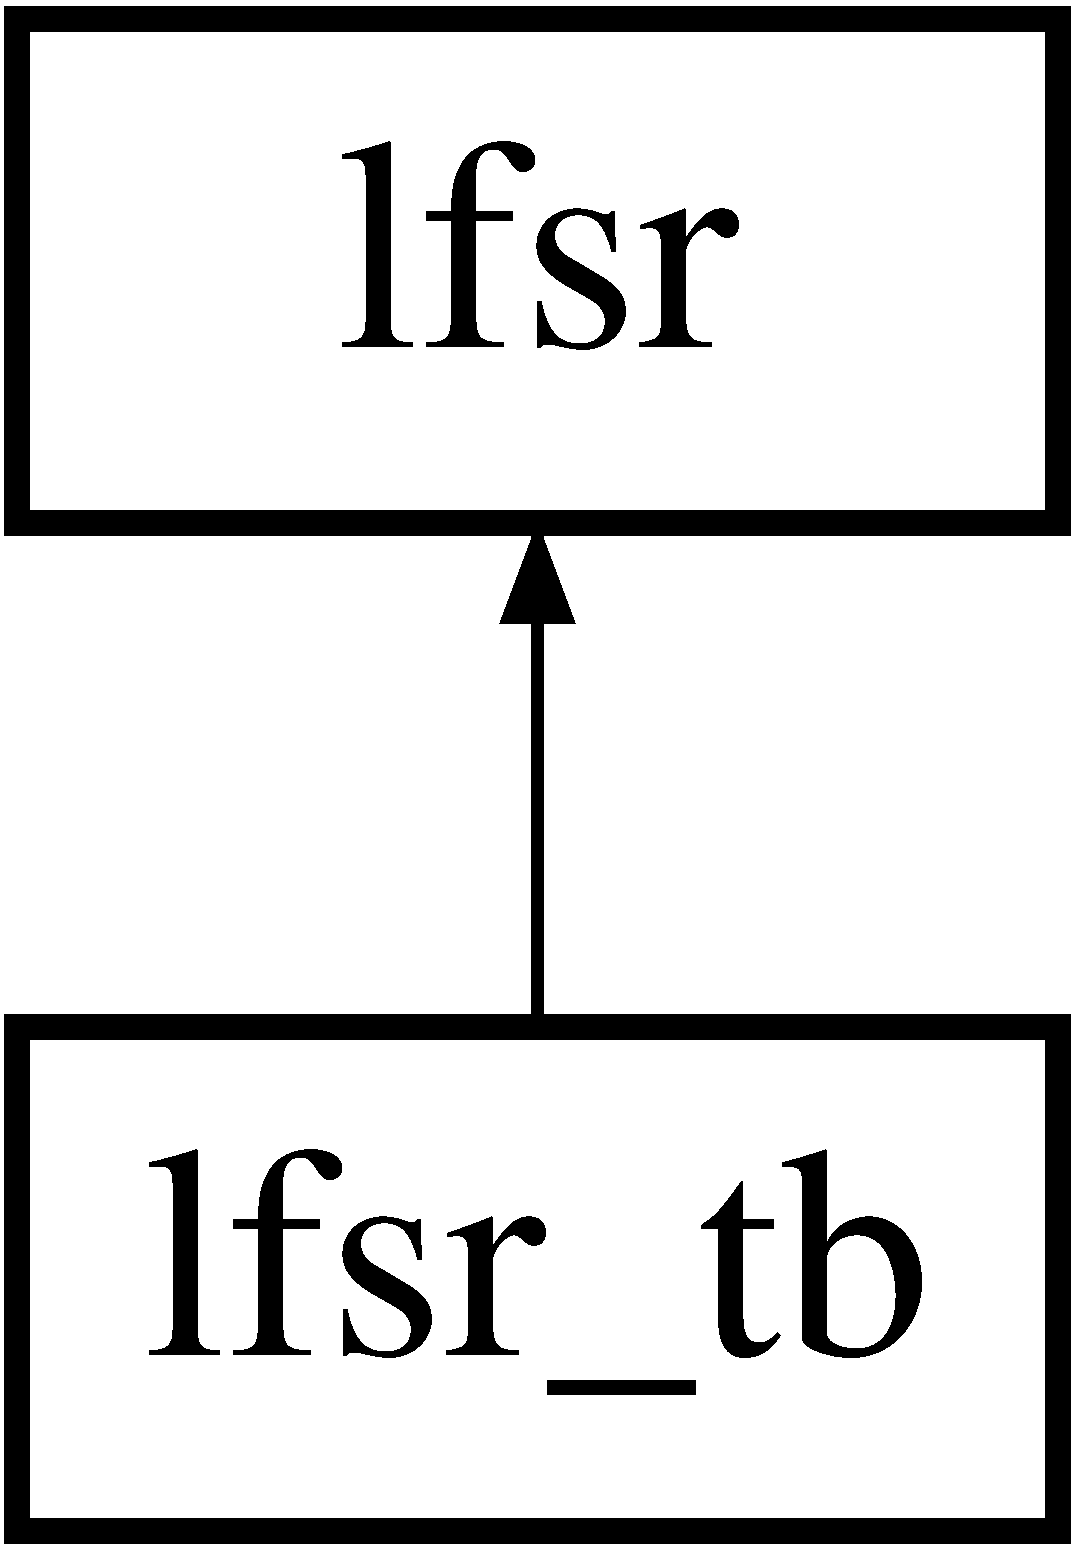
\includegraphics[height=2.000000cm]{classlfsr}
\end{center}
\end{figure}
\subsection*{Entities}
\begin{DoxyCompactItemize}
\item 
\hyperlink{classlfsr_1_1beh}{beh} architecture
\end{DoxyCompactItemize}
\subsection*{Use Clauses}
 \begin{DoxyCompactItemize}
\item 
\hypertarget{classlfsr_a2edc34402b573437d5f25fa90ba4013e}{\hyperlink{classlfsr_a2edc34402b573437d5f25fa90ba4013e}{numeric\-\_\-std}   }\label{classlfsr_a2edc34402b573437d5f25fa90ba4013e}

\end{DoxyCompactItemize}
\subsection*{Generics}
 \begin{DoxyCompactItemize}
\item 
\hypertarget{classlfsr_a2c127387ae125a873b1279f2cbc979b6}{\hyperlink{classlfsr_a2c127387ae125a873b1279f2cbc979b6}{I\-S\-\_\-\-G\-A\-L\-O\-I\-S} {\bfseries {\bfseries \textcolor{comment}{boolean}\textcolor{vhdlchar}{ }\textcolor{vhdlchar}{\-:}\textcolor{vhdlchar}{=}\textcolor{vhdlchar}{ }\textcolor{vhdlchar}{true}\textcolor{vhdlchar}{ }}}}\label{classlfsr_a2c127387ae125a873b1279f2cbc979b6}

\item 
\hypertarget{classlfsr_a2821e922ab193f166cc0b10bd22ee445}{\hyperlink{classlfsr_a2821e922ab193f166cc0b10bd22ee445}{I\-N\-T\-E\-R\-N\-A\-L\-\_\-\-S\-I\-Z\-E} {\bfseries {\bfseries \textcolor{vhdlchar}{positive}\textcolor{vhdlchar}{ }\textcolor{vhdlchar}{\-:}\textcolor{vhdlchar}{=}\textcolor{vhdlchar}{ } \textcolor{vhdldigit}{8} \textcolor{vhdlchar}{ }}}}\label{classlfsr_a2821e922ab193f166cc0b10bd22ee445}

\item 
\hypertarget{classlfsr_a0485b6a32e35f31b13bdd15470f0c857}{\hyperlink{classlfsr_a0485b6a32e35f31b13bdd15470f0c857}{S\-E\-E\-D} {\bfseries {\bfseries \textcolor{comment}{natural}\textcolor{vhdlchar}{ }\textcolor{vhdlchar}{\-:}\textcolor{vhdlchar}{=}\textcolor{vhdlchar}{ } \textcolor{vhdldigit}{1} \textcolor{vhdlchar}{ }}}}\label{classlfsr_a0485b6a32e35f31b13bdd15470f0c857}

\item 
\hypertarget{classlfsr_a231e58c20fc18458965941e4cbdbaeec}{\hyperlink{classlfsr_a231e58c20fc18458965941e4cbdbaeec}{U\-S\-E\-\_\-\-X\-N\-O\-R} {\bfseries {\bfseries \textcolor{comment}{boolean}\textcolor{vhdlchar}{ }\textcolor{vhdlchar}{\-:}\textcolor{vhdlchar}{=}\textcolor{vhdlchar}{ }\textcolor{vhdlchar}{true}\textcolor{vhdlchar}{ }}}}\label{classlfsr_a231e58c20fc18458965941e4cbdbaeec}

\item 
\hypertarget{classlfsr_af4d4b41e7c0bdda07e747bad04b9c5ef}{\hyperlink{classlfsr_af4d4b41e7c0bdda07e747bad04b9c5ef}{U\-S\-E\-\_\-\-C\-U\-S\-T\-O\-M\-\_\-\-P\-O\-L\-Y} {\bfseries {\bfseries \textcolor{comment}{boolean}\textcolor{vhdlchar}{ }\textcolor{vhdlchar}{\-:}\textcolor{vhdlchar}{=}\textcolor{vhdlchar}{ }\textcolor{vhdlchar}{false}\textcolor{vhdlchar}{ }}}}\label{classlfsr_af4d4b41e7c0bdda07e747bad04b9c5ef}

\item 
\hypertarget{classlfsr_a7d64141a514f3177a611abb7f25e6f6f}{\hyperlink{classlfsr_a7d64141a514f3177a611abb7f25e6f6f}{C\-U\-S\-T\-O\-M\-\_\-\-P\-O\-L\-Y} {\bfseries {\bfseries \textcolor{comment}{std\-\_\-logic\-\_\-vector}\textcolor{vhdlchar}{ }\textcolor{vhdlchar}{\-:}\textcolor{vhdlchar}{=}\textcolor{vhdlchar}{ }\textcolor{vhdlchar}{(}\textcolor{vhdlchar}{ }\textcolor{vhdlchar}{ } \textcolor{vhdldigit}{1} \textcolor{vhdlchar}{ }\textcolor{vhdlchar}{ }\textcolor{vhdlchar}{ }\textcolor{vhdlkeyword}{downto}\textcolor{vhdlchar}{ }\textcolor{vhdlchar}{ }\textcolor{vhdlchar}{ } \textcolor{vhdldigit}{0} \textcolor{vhdlchar}{ }\textcolor{vhdlchar}{ }\textcolor{vhdlchar}{=}\textcolor{vhdlchar}{ }\textcolor{vhdlchar}{$>$}\textcolor{vhdlchar}{ }\textcolor{vhdlchar}{'}\textcolor{vhdlchar}{ } \textcolor{vhdldigit}{0} \textcolor{vhdlchar}{ }\textcolor{vhdlchar}{'}\textcolor{vhdlchar}{ }\textcolor{vhdlchar}{ }\textcolor{vhdlchar}{)}\textcolor{vhdlchar}{ }}}}\label{classlfsr_a7d64141a514f3177a611abb7f25e6f6f}

\end{DoxyCompactItemize}
\subsection*{Ports}
 \begin{DoxyCompactItemize}
\item 
\hypertarget{classlfsr_aec59ad7fb872308b3e1a455c5328cdff}{\hyperlink{classlfsr_aec59ad7fb872308b3e1a455c5328cdff}{clk}  {\bfseries {\bfseries \textcolor{vhdlkeyword}{in}\textcolor{vhdlchar}{ }}} {\bfseries \textcolor{comment}{std\-\_\-logic}\textcolor{vhdlchar}{ }} }\label{classlfsr_aec59ad7fb872308b3e1a455c5328cdff}

\item 
\hypertarget{classlfsr_a5cf3e8e1cb15fcfc3619d8dc23942d9c}{\hyperlink{classlfsr_a5cf3e8e1cb15fcfc3619d8dc23942d9c}{rst}  {\bfseries {\bfseries \textcolor{vhdlkeyword}{in}\textcolor{vhdlchar}{ }}} {\bfseries \textcolor{comment}{std\-\_\-logic}\textcolor{vhdlchar}{ }} }\label{classlfsr_a5cf3e8e1cb15fcfc3619d8dc23942d9c}

\item 
\hypertarget{classlfsr_a4b652fca0dff23dedf468470a5d9142c}{\hyperlink{classlfsr_a4b652fca0dff23dedf468470a5d9142c}{q}  {\bfseries {\bfseries \textcolor{vhdlkeyword}{out}\textcolor{vhdlchar}{ }}} {\bfseries \textcolor{comment}{std\-\_\-logic\-\_\-vector}\textcolor{vhdlchar}{ }} }\label{classlfsr_a4b652fca0dff23dedf468470a5d9142c}

\end{DoxyCompactItemize}


The documentation for this class was generated from the following file\-:\begin{DoxyCompactItemize}
\item 
src/lfsr/lfsr.\-vhd\end{DoxyCompactItemize}

\hypertarget{classlfsr__internal}{\section{lfsr\-\_\-internal Entity Reference}
\label{classlfsr__internal}\index{lfsr\-\_\-internal@{lfsr\-\_\-internal}}
}
\subsection*{Entities}
\begin{DoxyCompactItemize}
\item 
\hyperlink{classlfsr__internal_1_1direct}{direct} architecture
\item 
\hyperlink{classlfsr__internal_1_1galois}{galois} architecture
\end{DoxyCompactItemize}
\subsection*{Libraries}
 \begin{DoxyCompactItemize}
\item 
\hypertarget{classlfsr__internal_af4aebbb5387a0e68735d64561e96bb77}{\hyperlink{classlfsr__internal_af4aebbb5387a0e68735d64561e96bb77}{Boost\-D\-S\-P} }\label{classlfsr__internal_af4aebbb5387a0e68735d64561e96bb77}

\end{DoxyCompactItemize}
\subsection*{Use Clauses}
 \begin{DoxyCompactItemize}
\item 
\hypertarget{classlfsr__internal_a2edc34402b573437d5f25fa90ba4013e}{\hyperlink{classlfsr__internal_a2edc34402b573437d5f25fa90ba4013e}{numeric\-\_\-std}   }\label{classlfsr__internal_a2edc34402b573437d5f25fa90ba4013e}

\item 
\hypertarget{classlfsr__internal_a4aaca332b2340a63e969ac63f1ba3e5d}{\hyperlink{classlfsr__internal_a4aaca332b2340a63e969ac63f1ba3e5d}{util\-\_\-pkg}   }\label{classlfsr__internal_a4aaca332b2340a63e969ac63f1ba3e5d}

\item 
\hypertarget{classlfsr__internal_adb085513a5228f37a5a2d9e04d8bdf76}{\hyperlink{classlfsr__internal_adb085513a5228f37a5a2d9e04d8bdf76}{lfsr\-\_\-pkg}   }\label{classlfsr__internal_adb085513a5228f37a5a2d9e04d8bdf76}

\end{DoxyCompactItemize}
\subsection*{Generics}
 \begin{DoxyCompactItemize}
\item 
\hypertarget{classlfsr__internal_a2821e922ab193f166cc0b10bd22ee445}{\hyperlink{classlfsr__internal_a2821e922ab193f166cc0b10bd22ee445}{I\-N\-T\-E\-R\-N\-A\-L\-\_\-\-S\-I\-Z\-E} {\bfseries {\bfseries \textcolor{vhdlchar}{positive}\textcolor{vhdlchar}{ }\textcolor{vhdlchar}{\-:}\textcolor{vhdlchar}{=}\textcolor{vhdlchar}{ } \textcolor{vhdldigit}{8} \textcolor{vhdlchar}{ }}}}\label{classlfsr__internal_a2821e922ab193f166cc0b10bd22ee445}

\item 
\hypertarget{classlfsr__internal_a0485b6a32e35f31b13bdd15470f0c857}{\hyperlink{classlfsr__internal_a0485b6a32e35f31b13bdd15470f0c857}{S\-E\-E\-D} {\bfseries {\bfseries \textcolor{comment}{natural}\textcolor{vhdlchar}{ }\textcolor{vhdlchar}{\-:}\textcolor{vhdlchar}{=}\textcolor{vhdlchar}{ } \textcolor{vhdldigit}{1} \textcolor{vhdlchar}{ }}}}\label{classlfsr__internal_a0485b6a32e35f31b13bdd15470f0c857}

\item 
\hypertarget{classlfsr__internal_a231e58c20fc18458965941e4cbdbaeec}{\hyperlink{classlfsr__internal_a231e58c20fc18458965941e4cbdbaeec}{U\-S\-E\-\_\-\-X\-N\-O\-R} {\bfseries {\bfseries \textcolor{comment}{boolean}\textcolor{vhdlchar}{ }\textcolor{vhdlchar}{\-:}\textcolor{vhdlchar}{=}\textcolor{vhdlchar}{ }\textcolor{vhdlchar}{true}\textcolor{vhdlchar}{ }}}}\label{classlfsr__internal_a231e58c20fc18458965941e4cbdbaeec}

\item 
\hypertarget{classlfsr__internal_af4d4b41e7c0bdda07e747bad04b9c5ef}{\hyperlink{classlfsr__internal_af4d4b41e7c0bdda07e747bad04b9c5ef}{U\-S\-E\-\_\-\-C\-U\-S\-T\-O\-M\-\_\-\-P\-O\-L\-Y} {\bfseries {\bfseries \textcolor{comment}{boolean}\textcolor{vhdlchar}{ }\textcolor{vhdlchar}{\-:}\textcolor{vhdlchar}{=}\textcolor{vhdlchar}{ }\textcolor{vhdlchar}{false}\textcolor{vhdlchar}{ }}}}\label{classlfsr__internal_af4d4b41e7c0bdda07e747bad04b9c5ef}

\item 
\hypertarget{classlfsr__internal_a7d64141a514f3177a611abb7f25e6f6f}{\hyperlink{classlfsr__internal_a7d64141a514f3177a611abb7f25e6f6f}{C\-U\-S\-T\-O\-M\-\_\-\-P\-O\-L\-Y} {\bfseries {\bfseries \textcolor{comment}{std\-\_\-logic\-\_\-vector}\textcolor{vhdlchar}{ }\textcolor{vhdlchar}{\-:}\textcolor{vhdlchar}{=}\textcolor{vhdlchar}{ }\textcolor{vhdlchar}{(}\textcolor{vhdlchar}{ }\textcolor{vhdlchar}{ } \textcolor{vhdldigit}{1} \textcolor{vhdlchar}{ }\textcolor{vhdlchar}{ }\textcolor{vhdlchar}{ }\textcolor{vhdlkeyword}{downto}\textcolor{vhdlchar}{ }\textcolor{vhdlchar}{ }\textcolor{vhdlchar}{ } \textcolor{vhdldigit}{0} \textcolor{vhdlchar}{ }\textcolor{vhdlchar}{ }\textcolor{vhdlchar}{=}\textcolor{vhdlchar}{ }\textcolor{vhdlchar}{$>$}\textcolor{vhdlchar}{ }\textcolor{vhdlchar}{'}\textcolor{vhdlchar}{ } \textcolor{vhdldigit}{0} \textcolor{vhdlchar}{ }\textcolor{vhdlchar}{'}\textcolor{vhdlchar}{ }\textcolor{vhdlchar}{ }\textcolor{vhdlchar}{)}\textcolor{vhdlchar}{ }}}}\label{classlfsr__internal_a7d64141a514f3177a611abb7f25e6f6f}

\end{DoxyCompactItemize}
\subsection*{Ports}
 \begin{DoxyCompactItemize}
\item 
\hypertarget{classlfsr__internal_aec59ad7fb872308b3e1a455c5328cdff}{\hyperlink{classlfsr__internal_aec59ad7fb872308b3e1a455c5328cdff}{clk}  {\bfseries {\bfseries \textcolor{vhdlkeyword}{in}\textcolor{vhdlchar}{ }}} {\bfseries \textcolor{comment}{std\-\_\-logic}\textcolor{vhdlchar}{ }} }\label{classlfsr__internal_aec59ad7fb872308b3e1a455c5328cdff}

\item 
\hypertarget{classlfsr__internal_a5cf3e8e1cb15fcfc3619d8dc23942d9c}{\hyperlink{classlfsr__internal_a5cf3e8e1cb15fcfc3619d8dc23942d9c}{rst}  {\bfseries {\bfseries \textcolor{vhdlkeyword}{in}\textcolor{vhdlchar}{ }}} {\bfseries \textcolor{comment}{std\-\_\-logic}\textcolor{vhdlchar}{ }} }\label{classlfsr__internal_a5cf3e8e1cb15fcfc3619d8dc23942d9c}

\item 
\hypertarget{classlfsr__internal_a4b652fca0dff23dedf468470a5d9142c}{\hyperlink{classlfsr__internal_a4b652fca0dff23dedf468470a5d9142c}{q}  {\bfseries {\bfseries \textcolor{vhdlkeyword}{out}\textcolor{vhdlchar}{ }}} {\bfseries \textcolor{comment}{std\-\_\-logic\-\_\-vector}\textcolor{vhdlchar}{ }} }\label{classlfsr__internal_a4b652fca0dff23dedf468470a5d9142c}

\end{DoxyCompactItemize}


The documentation for this class was generated from the following file\-:\begin{DoxyCompactItemize}
\item 
src/lfsr/lfsr\-\_\-internal\-\_\-ea.\-vhd\end{DoxyCompactItemize}

\hypertarget{classlfsr__pkg}{\section{lfsr\-\_\-pkg Package Reference}
\label{classlfsr__pkg}\index{lfsr\-\_\-pkg@{lfsr\-\_\-pkg}}
}
{\bfseries Package Body $>$$>$ }\hyperlink{class__lfsr__pkg}{lfsr\-\_\-pkg}\\*
\subsection*{Functions}
 \begin{DoxyCompactItemize}
\item 
\hypertarget{classlfsr__pkg_aa892d93dafd63bb0a40765dec3e73940}{{\bfseries {\bfseries \textcolor{comment}{std\-\_\-logic\-\_\-vector}\textcolor{vhdlchar}{ }}} \hyperlink{classlfsr__pkg_aa892d93dafd63bb0a40765dec3e73940}{Maximal\-\_\-\-Polynomial}{\bfseries  ( }{\bfseries \textcolor{vhdlchar}{size\-: }\textcolor{stringliteral}{in }\textcolor{vhdlchar}{positive}}{\bfseries  )} }\label{classlfsr__pkg_aa892d93dafd63bb0a40765dec3e73940}

\end{DoxyCompactItemize}


The documentation for this class was generated from the following file\-:\begin{DoxyCompactItemize}
\item 
src/lfsr/lfsr\-\_\-pkg.\-vhd\end{DoxyCompactItemize}

\hypertarget{classlfsr__tb}{\section{lfsr\-\_\-tb Entity Reference}
\label{classlfsr__tb}\index{lfsr\-\_\-tb@{lfsr\-\_\-tb}}
}
Inheritance diagram for lfsr\-\_\-tb\-:\begin{figure}[H]
\begin{center}
\leavevmode
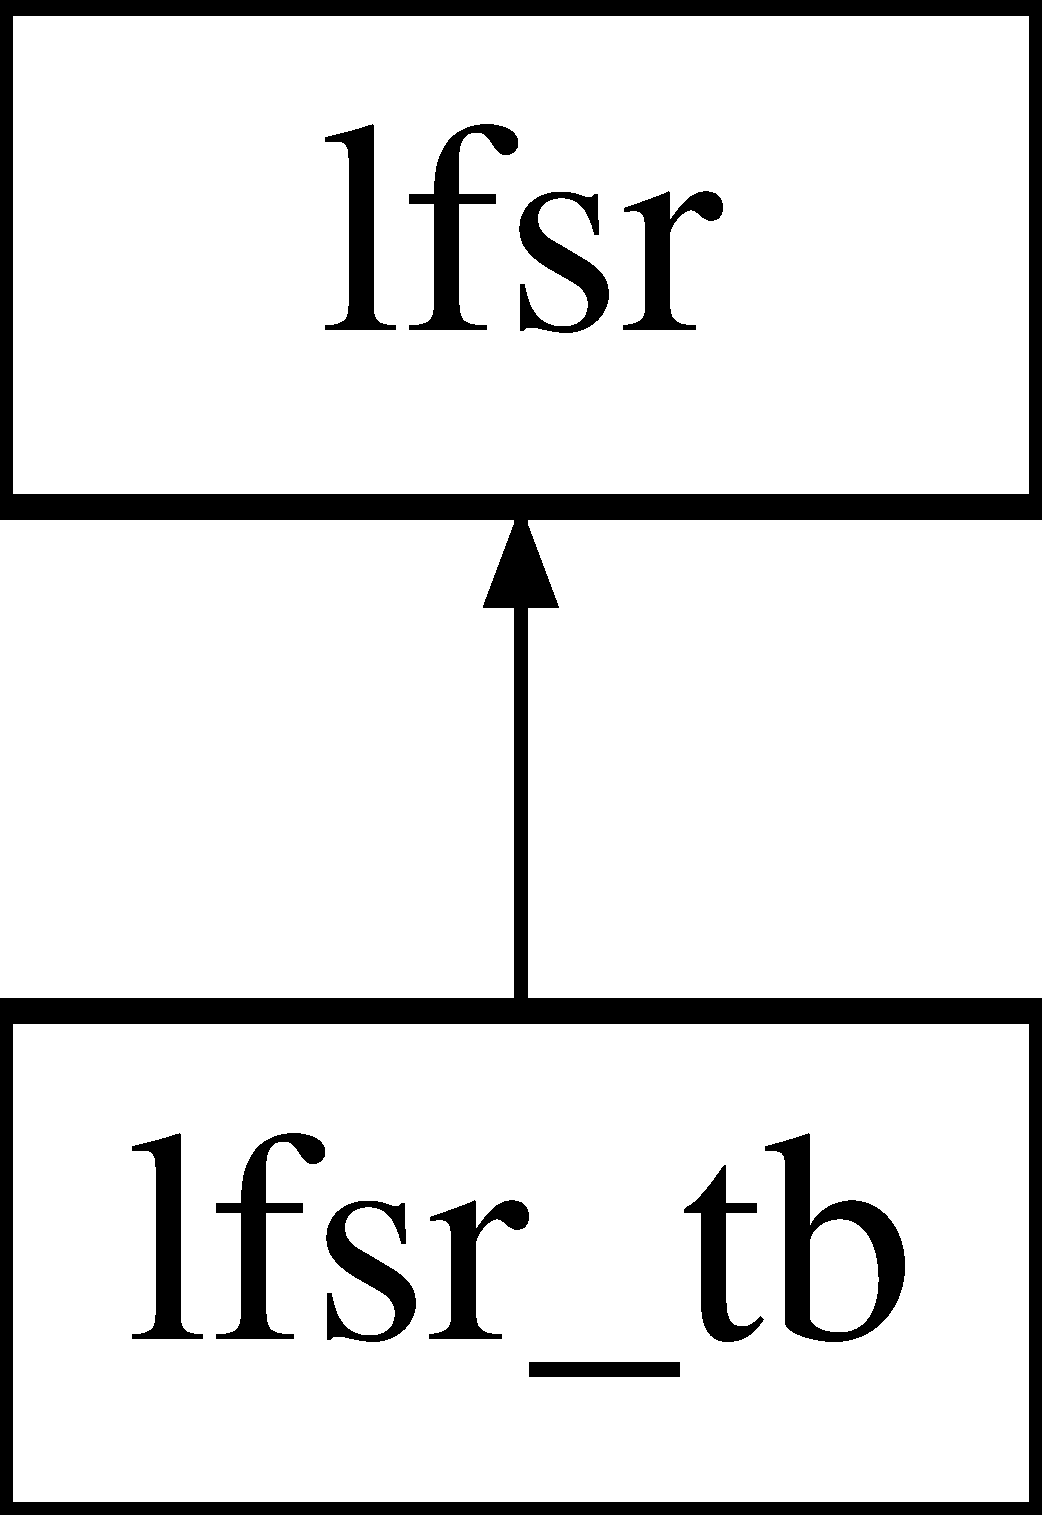
\includegraphics[height=2.000000cm]{classlfsr__tb}
\end{center}
\end{figure}
\subsection*{Entities}
\begin{DoxyCompactItemize}
\item 
\hyperlink{classlfsr__tb_1_1sim}{sim} architecture
\end{DoxyCompactItemize}
\subsection*{Use Clauses}
 \begin{DoxyCompactItemize}
\item 
\hypertarget{classlfsr__tb_a2edc34402b573437d5f25fa90ba4013e}{\hyperlink{classlfsr__tb_a2edc34402b573437d5f25fa90ba4013e}{numeric\-\_\-std}   }\label{classlfsr__tb_a2edc34402b573437d5f25fa90ba4013e}

\item 
\hypertarget{classlfsr__tb_aa8c4e25998323a84db5b1fa701b92fcb}{\hyperlink{classlfsr__tb_aa8c4e25998323a84db5b1fa701b92fcb}{textio}   }\label{classlfsr__tb_aa8c4e25998323a84db5b1fa701b92fcb}

\end{DoxyCompactItemize}
\subsection*{Generics}
 \begin{DoxyCompactItemize}
\item 
\hypertarget{classlfsr__tb_a7dd564a173315445201d6e4a97b36a64}{\hyperlink{classlfsr__tb_a7dd564a173315445201d6e4a97b36a64}{L\-F\-S\-R\-\_\-\-L\-E\-N\-G\-T\-H} {\bfseries {\bfseries \textcolor{vhdlchar}{positive}\textcolor{vhdlchar}{ }\textcolor{vhdlchar}{\-:}\textcolor{vhdlchar}{=}\textcolor{vhdlchar}{ } \textcolor{vhdldigit}{8} \textcolor{vhdlchar}{ }}}}\label{classlfsr__tb_a7dd564a173315445201d6e4a97b36a64}

\item 
\hypertarget{classlfsr__tb_ae5f49eba61f25213abee8b3c9f9e41cc}{\hyperlink{classlfsr__tb_ae5f49eba61f25213abee8b3c9f9e41cc}{D\-U\-M\-P\-\_\-\-F\-I\-L\-E} {\bfseries {\bfseries \textcolor{comment}{string}\textcolor{vhdlchar}{ }\textcolor{vhdlchar}{\-:}\textcolor{vhdlchar}{=}\textcolor{vhdlchar}{ }\textcolor{comment}{string}\textcolor{vhdlchar}{ }\textcolor{vhdlchar}{'}\textcolor{vhdlchar}{ }\textcolor{vhdlchar}{(}\textcolor{vhdlchar}{ }\textcolor{keyword}{\char`\"{} lfsr\-\_\-dump.\-txt \char`\"{}}\textcolor{vhdlchar}{ }\textcolor{vhdlchar}{ }\textcolor{vhdlchar}{)}\textcolor{vhdlchar}{ }}}}\label{classlfsr__tb_ae5f49eba61f25213abee8b3c9f9e41cc}

\end{DoxyCompactItemize}


The documentation for this class was generated from the following file\-:\begin{DoxyCompactItemize}
\item 
src/lfsr/lfsr\-\_\-tb.\-vhd\end{DoxyCompactItemize}

\hypertarget{classlfsr__tb_1_1sim}{\section{sim Architecture Reference}
\label{classlfsr__tb_1_1sim}\index{sim@{sim}}
}
\subsection*{Processes}
 \begin{DoxyCompactItemize}
\item 
\hypertarget{classlfsr__tb_1_1sim_a47d2864b6dd82daccd7b71fcfd9a682c}{\hyperlink{classlfsr__tb_1_1sim_a47d2864b6dd82daccd7b71fcfd9a682c}{clk\-\_\-gen}{\bfseries  (  )}}\label{classlfsr__tb_1_1sim_a47d2864b6dd82daccd7b71fcfd9a682c}

\item 
\hypertarget{classlfsr__tb_1_1sim_ac384adbd9df3496973e9349fd5ca6900}{\hyperlink{classlfsr__tb_1_1sim_ac384adbd9df3496973e9349fd5ca6900}{rst\-\_\-proc}{\bfseries  (  )}}\label{classlfsr__tb_1_1sim_ac384adbd9df3496973e9349fd5ca6900}

\item 
\hypertarget{classlfsr__tb_1_1sim_a6523adb14d9acd35e5ec8df5867a6a36}{\hyperlink{classlfsr__tb_1_1sim_a6523adb14d9acd35e5ec8df5867a6a36}{record\-\_\-output}{\bfseries  (  )}}\label{classlfsr__tb_1_1sim_a6523adb14d9acd35e5ec8df5867a6a36}

\item 
\hypertarget{classlfsr__tb_1_1sim_a35ccef32cc961f4b28be03e498532eb3}{\hyperlink{classlfsr__tb_1_1sim_a35ccef32cc961f4b28be03e498532eb3}{check\-\_\-states}{\bfseries  (  )}}\label{classlfsr__tb_1_1sim_a35ccef32cc961f4b28be03e498532eb3}

\end{DoxyCompactItemize}
\subsection*{Components}
 \begin{DoxyCompactItemize}
\item 
\hypertarget{classlfsr__tb_1_1sim_aabe8f8d9ad34874edd366edaf2e00cc0}{\hyperlink{classlfsr__tb_1_1sim_aabe8f8d9ad34874edd366edaf2e00cc0}{lfsr}  {\bfseries }  }\label{classlfsr__tb_1_1sim_aabe8f8d9ad34874edd366edaf2e00cc0}

\end{DoxyCompactItemize}
\subsection*{Constants}
 \begin{DoxyCompactItemize}
\item 
\hypertarget{classlfsr__tb_1_1sim_ac1dd4fc6ce65755e29c83ff9b8609367}{\hyperlink{classlfsr__tb_1_1sim_ac1dd4fc6ce65755e29c83ff9b8609367}{clk\-\_\-p} {\bfseries \textcolor{comment}{time}\textcolor{vhdlchar}{ }\textcolor{vhdlchar}{ }\textcolor{vhdlchar}{\-:}\textcolor{vhdlchar}{=}\textcolor{vhdlchar}{ } \textcolor{vhdldigit}{2} \textcolor{vhdlchar}{ }\textcolor{vhdlchar}{ns}\textcolor{vhdlchar}{ }} }\label{classlfsr__tb_1_1sim_ac1dd4fc6ce65755e29c83ff9b8609367}

\item 
\hypertarget{classlfsr__tb_1_1sim_a7bde034fc12da33af41742f87897771b}{\hyperlink{classlfsr__tb_1_1sim_a7bde034fc12da33af41742f87897771b}{A\-L\-L\-\_\-\-C\-H\-O\-S\-E\-N} {\bfseries \textcolor{comment}{std\-\_\-logic\-\_\-vector}\textcolor{vhdlchar}{ }\textcolor{vhdlchar}{(}\textcolor{vhdlchar}{ }\textcolor{vhdlchar}{ }\textcolor{vhdlchar}{chosen}\textcolor{vhdlchar}{ }\textcolor{vhdlchar}{'}\textcolor{vhdlchar}{ }\textcolor{vhdlchar}{ }\textcolor{vhdlkeyword}{range}\textcolor{vhdlchar}{ }\textcolor{vhdlchar}{ }\textcolor{vhdlchar}{)}\textcolor{vhdlchar}{ }\textcolor{vhdlchar}{ }\textcolor{vhdlchar}{\-:}\textcolor{vhdlchar}{=}\textcolor{vhdlchar}{ }\textcolor{vhdlchar}{(}\textcolor{vhdlchar}{ }\textcolor{vhdlchar}{ }\textcolor{vhdlkeyword}{others}\textcolor{vhdlchar}{ }\textcolor{vhdlchar}{ }\textcolor{vhdlchar}{=}\textcolor{vhdlchar}{ }\textcolor{vhdlchar}{$>$}\textcolor{vhdlchar}{ }\textcolor{vhdlchar}{'}\textcolor{vhdlchar}{ } \textcolor{vhdldigit}{1} \textcolor{vhdlchar}{ }\textcolor{vhdlchar}{'}\textcolor{vhdlchar}{ }\textcolor{vhdlchar}{ }\textcolor{vhdlchar}{)}\textcolor{vhdlchar}{ }} }\label{classlfsr__tb_1_1sim_a7bde034fc12da33af41742f87897771b}

\end{DoxyCompactItemize}
\subsection*{Signals}
 \begin{DoxyCompactItemize}
\item 
\hypertarget{classlfsr__tb_1_1sim_a956914b9d3dc0b7b0d06190fd8c4d35c}{\hyperlink{classlfsr__tb_1_1sim_a956914b9d3dc0b7b0d06190fd8c4d35c}{clk} {\bfseries \textcolor{comment}{std\-\_\-logic}\textcolor{vhdlchar}{ }\textcolor{vhdlchar}{ }\textcolor{vhdlchar}{\-:}\textcolor{vhdlchar}{=}\textcolor{vhdlchar}{ }\textcolor{vhdlchar}{'}\textcolor{vhdlchar}{ } \textcolor{vhdldigit}{0} \textcolor{vhdlchar}{ }\textcolor{vhdlchar}{'}\textcolor{vhdlchar}{ }} }\label{classlfsr__tb_1_1sim_a956914b9d3dc0b7b0d06190fd8c4d35c}

\item 
\hypertarget{classlfsr__tb_1_1sim_ae31155b42b9c6b307df946da31307d64}{\hyperlink{classlfsr__tb_1_1sim_ae31155b42b9c6b307df946da31307d64}{rst} {\bfseries \textcolor{comment}{std\-\_\-logic}\textcolor{vhdlchar}{ }\textcolor{vhdlchar}{ }\textcolor{vhdlchar}{\-:}\textcolor{vhdlchar}{=}\textcolor{vhdlchar}{ }\textcolor{vhdlchar}{'}\textcolor{vhdlchar}{ } \textcolor{vhdldigit}{0} \textcolor{vhdlchar}{ }\textcolor{vhdlchar}{'}\textcolor{vhdlchar}{ }} }\label{classlfsr__tb_1_1sim_ae31155b42b9c6b307df946da31307d64}

\item 
\hypertarget{classlfsr__tb_1_1sim_a367866422ab940c485a863d828f09a47}{\hyperlink{classlfsr__tb_1_1sim_a367866422ab940c485a863d828f09a47}{q} {\bfseries \textcolor{comment}{std\-\_\-logic\-\_\-vector}\textcolor{vhdlchar}{ }\textcolor{vhdlchar}{(}\textcolor{vhdlchar}{ }\textcolor{vhdlchar}{ }\textcolor{vhdlchar}{(}\textcolor{vhdlchar}{ }\textcolor{vhdlchar}{L\-F\-S\-R\-\_\-\-L\-E\-N\-G\-T\-H}\textcolor{vhdlchar}{ }\textcolor{vhdlchar}{-\/}\textcolor{vhdlchar}{ } \textcolor{vhdldigit}{1} \textcolor{vhdlchar}{ }\textcolor{vhdlchar}{)}\textcolor{vhdlchar}{ }\textcolor{vhdlchar}{ }\textcolor{vhdlchar}{ }\textcolor{vhdlchar}{ }\textcolor{vhdlkeyword}{downto}\textcolor{vhdlchar}{ }\textcolor{vhdlchar}{ }\textcolor{vhdlchar}{ } \textcolor{vhdldigit}{0} \textcolor{vhdlchar}{ }\textcolor{vhdlchar}{)}\textcolor{vhdlchar}{ }} }\label{classlfsr__tb_1_1sim_a367866422ab940c485a863d828f09a47}

\item 
\hypertarget{classlfsr__tb_1_1sim_a8af801aefd2ca7b2d72e2dad0b151d5d}{\hyperlink{classlfsr__tb_1_1sim_a8af801aefd2ca7b2d72e2dad0b151d5d}{chosen} {\bfseries \textcolor{comment}{std\-\_\-logic\-\_\-vector}\textcolor{vhdlchar}{ }\textcolor{vhdlchar}{(}\textcolor{vhdlchar}{ }\textcolor{vhdlchar}{ }\textcolor{vhdlchar}{(}\textcolor{vhdlchar}{ }\textcolor{vhdlchar}{(}\textcolor{vhdlchar}{ } \textcolor{vhdldigit}{2} \textcolor{vhdlchar}{ }\textcolor{vhdlchar}{$\ast$}\textcolor{vhdlchar}{$\ast$}\textcolor{vhdlchar}{ }\textcolor{vhdlchar}{q}\textcolor{vhdlchar}{ }\textcolor{vhdlchar}{'}\textcolor{vhdlchar}{ }\textcolor{vhdlchar}{ }\textcolor{vhdlchar}{length}\textcolor{vhdlchar}{ }\textcolor{vhdlchar}{)}\textcolor{vhdlchar}{ }\textcolor{vhdlchar}{ }\textcolor{vhdlchar}{-\/}\textcolor{vhdlchar}{ } \textcolor{vhdldigit}{2} \textcolor{vhdlchar}{ }\textcolor{vhdlchar}{)}\textcolor{vhdlchar}{ }\textcolor{vhdlchar}{ }\textcolor{vhdlchar}{ }\textcolor{vhdlchar}{ }\textcolor{vhdlkeyword}{downto}\textcolor{vhdlchar}{ }\textcolor{vhdlchar}{ }\textcolor{vhdlchar}{ } \textcolor{vhdldigit}{0} \textcolor{vhdlchar}{ }\textcolor{vhdlchar}{)}\textcolor{vhdlchar}{ }} }\label{classlfsr__tb_1_1sim_a8af801aefd2ca7b2d72e2dad0b151d5d}

\end{DoxyCompactItemize}
\subsection*{Files}
 \begin{DoxyCompactItemize}
\item 
\hypertarget{classlfsr__tb_1_1sim_a0fcbb6d242fd50c6a09138675a054a78}{\hyperlink{classlfsr__tb_1_1sim_a0fcbb6d242fd50c6a09138675a054a78}{dump} {\bfseries \textcolor{vhdlchar}{text}\textcolor{vhdlchar}{ }\textcolor{vhdlkeyword}{open}\textcolor{vhdlchar}{ }\textcolor{vhdlchar}{write\-\_\-mode}\textcolor{vhdlchar}{ }\textcolor{vhdlkeyword}{is}\textcolor{vhdlchar}{ }\textcolor{vhdlchar}{D\-U\-M\-P\-\_\-\-F\-I\-L\-E}\textcolor{vhdlchar}{ }} }\label{classlfsr__tb_1_1sim_a0fcbb6d242fd50c6a09138675a054a78}

\end{DoxyCompactItemize}
\subsection*{Instantiations}
 \begin{DoxyCompactItemize}
\item 
\hypertarget{classlfsr__tb_1_1sim_a1619316ad715601eb5d3559db829ac05}{\hyperlink{classlfsr__tb_1_1sim_a1619316ad715601eb5d3559db829ac05}{uut}  {\bfseries lfsr}   }\label{classlfsr__tb_1_1sim_a1619316ad715601eb5d3559db829ac05}

\end{DoxyCompactItemize}


The documentation for this class was generated from the following files\-:\begin{DoxyCompactItemize}
\item 
src/lfsr/lfsr\-\_\-tb.\-vhd\end{DoxyCompactItemize}

\hypertarget{classutil__pkg}{\section{util\-\_\-pkg Package Reference}
\label{classutil__pkg}\index{util\-\_\-pkg@{util\-\_\-pkg}}
}
{\bfseries Package Body $>$$>$ }\hyperlink{class__util__pkg}{util\-\_\-pkg}\\*
\subsection*{Functions}
 \begin{DoxyCompactItemize}
\item 
\hypertarget{classutil__pkg_a75d57d42f413f4f44fe472e114c76b50}{{\bfseries {\bfseries \textcolor{comment}{integer}\textcolor{vhdlchar}{ }}} \hyperlink{classutil__pkg_a75d57d42f413f4f44fe472e114c76b50}{max}{\bfseries  ( }{\bfseries \textcolor{vhdlchar}{i\-: }\textcolor{stringliteral}{in }{\bfseries \textcolor{comment}{integer}\textcolor{vhdlchar}{ }}}{\bfseries  , \textcolor{vhdlchar}{j\-: }\textcolor{stringliteral}{in }{\bfseries \textcolor{comment}{integer}\textcolor{vhdlchar}{ }}}{\bfseries  )} }\label{classutil__pkg_a75d57d42f413f4f44fe472e114c76b50}

\item 
\hypertarget{classutil__pkg_a9abf89c3351a7e2c76ffa1943ab815e0}{{\bfseries {\bfseries \textcolor{comment}{std\-\_\-logic\-\_\-vector}\textcolor{vhdlchar}{ }}} \hyperlink{classutil__pkg_a9abf89c3351a7e2c76ffa1943ab815e0}{reverse}{\bfseries  ( }{\bfseries \textcolor{vhdlchar}{x\-: }\textcolor{stringliteral}{in }{\bfseries \textcolor{comment}{std\-\_\-logic\-\_\-vector}\textcolor{vhdlchar}{ }}}{\bfseries  )} }\label{classutil__pkg_a9abf89c3351a7e2c76ffa1943ab815e0}

\end{DoxyCompactItemize}
\subsection*{Use Clauses}
 \begin{DoxyCompactItemize}
\item 
\hypertarget{classutil__pkg_a2edc34402b573437d5f25fa90ba4013e}{\hyperlink{classutil__pkg_a2edc34402b573437d5f25fa90ba4013e}{numeric\-\_\-std}   }\label{classutil__pkg_a2edc34402b573437d5f25fa90ba4013e}

\end{DoxyCompactItemize}


The documentation for this class was generated from the following file\-:\begin{DoxyCompactItemize}
\item 
src/util\-\_\-pkg.\-vhd\end{DoxyCompactItemize}

\addcontentsline{toc}{part}{Index}
\printindex
\end{document}
